\documentclass[a4paper,11pt,onecolumn,twoside]{article}
\usepackage{ctex}
\usepackage{times}
\usepackage{setspace}
\usepackage{fancyhdr}
\usepackage{graphicx}
\usepackage{subfigure}
\usepackage{wrapfig}
\usepackage{array}  
\usepackage{fontspec,xunicode,xltxtra}
\usepackage{titlesec}
\usepackage{titletoc}
\usepackage[titletoc]{appendix}
\usepackage[hyphens]{url}
\usepackage{cite}
\usepackage{listings}

%%%%%%%%%%%%%%%%%%%%%%%%%%%%%%%%%%%%%%%%%%%%%%%%%%%%%%%%%%%%%%%%
%  lengths
%    下面的命令重定义页面边距,使其符合中文刊物习惯。
%%%%%%%%%%%%%%%%%%%%%%%%%%%%%%%%%%%%%%%%%%%%%%%%%%%%%%%%%%%%%%%%
\addtolength{\topmargin}{-54pt}
\setlength{\oddsidemargin}{-0.9cm}  % 3.17cm - 1 inch
\setlength{\evensidemargin}{\oddsidemargin}
\setlength{\textwidth}{17.00cm}
\setlength{\textheight}{24.00cm}    % 24.62


\makeatletter
\newenvironment{figurehere}
  {\def\@captype{figure}}
  {}
\makeatother

%---------------------------------------------------------------------
%	引用文献设置为上标
%---------------------------------------------------------------------
\newcommand{\supercite}[1]{\textsuperscript{\cite{#1}}}



\begin{document}

\begin{titlepage}
	\begin{center}
		
    \vspace{4in}
    \phantom{anything}
        \textbf{\zihao{2}\heiti{任务一:最长密码}}\\
        \vspace{0.3in}
        \textbf{\zihao{3}\heiti{课程90:2015年Instant Prime挑战赛任务}}\\
    
	\vspace{\fill}
	
\setlength{\extrarowheight}{3mm}
{\songti\zihao{-3}	
\begin{tabular}{cc}
	
    {\makebox[6\ccwd][s]{项目来源:}}&~{软件工程导论课程}\\
    {\makebox[6\ccwd][s]{姓\qquad\quad 名:}}&~\kaishu{石广钊}\\ 
    {\makebox[6\ccwd][s]{学\qquad\quad 号:}}&~\kaishu{161180111}\\
    {\makebox[6\ccwd][s]{指导老师:}}&~\kaishu{方\qquad 晖}\\

\end{tabular}
 }\\[2cm]
	\end{center}	
\end{titlepage}

\tableofcontents % 生成目录
\clearpage


% \begin{center}
    {\heiti\zihao{2}\textbf{实验三\quad 复阻抗测量实验报告}}\\  
    {\centerline{\kaishu\zihao{5} (电子信息科学与技术 \qquad 石广钊 \qquad 161180111)}}  
\end{center}


\begin{spacing}{1.5}
\songti\zihao{-4}
% \setcounter{page}{1}
    \section{项目简介}
    \subsection{背景}
    本项目为南京大学电子学院《软件工程导学》课程作业。项目来源于为Codility.com网站 Lesson 90: Tasks from Indeed Prime 2015 challenge中的任务1。 
    项目要求写一个程序实现题目中要求的功能,编程语言不限,且本题对时间复杂读没有要求,只需保证正确性即可。

    \subsection{目的}
    项目要求设计一个函数,对于输入字符串S,返回其中符合密码要求的最长word的长度。其中不同word之间以空格分割,word可作为密码格式需满足三个条件,即:
    \begin{enumerate} [\indent (1)]
            \item 仅包含字母或数字字符(A\-Z, a\-z, 0\-9)。
            \item 需要包含偶数个字母(0,2,4,..)。
            \item 需要包含奇数个数字(1,3,5,..)。
    \end{enumerate}

    实现该功能的编程语言不限,字符串S长度N长度在[1..200]之间。
    
    \section{范围}
    本项目中,需要实现一个函数:

\begin{lstlisting}{language=C}
int solution(char *S)
\end{lstlisting}

    编写所得程序可以先通过自己编写的程序进行测试,再通过 codility.com 网站进行测试。

    \section{需求说明}
    \subsection{需求定义}
    \begin{enumerate} [\indent 1、]
        \item 程序能够根据空格位置分割输入的字符串。
        \item 程序能够判断字符串结束的位置。
        \item 程序能够检测一个word是否满足作为密码的三个条件。
        \item 程序可以返回最长密码的长度,如不存在满足要求的word,则返回-1。
        \item 保证返回长度的正确性。
    \end{enumerate}

    \subsection{需求规格说明}
    \begin{enumerate} [\indent 1、]
        \item 程序中使用切片函数将输入字符串分为多个字符串,或者直接遍字符串逐个处理字符。
        \item 若遇到空字符NULL表示字符串即结束,停止字符串遍历。
        \item 通过将字符的ASCII值与相应范围的数字比较判定字符是否符合要求,统计个字符数量即可判断是否符合要求。
        \item 对不同测试集进行测试来检测结果的正确性。
    \end{enumerate}
    
    \subsection{设计标准}
    评分系统:

    10--9 = 非常重要(必须完成)
    
    8--7 = 比较重要(能完成最好)
    
    6--4 = 重要而不必要(完成最好但是没有必要)
    
    3--0 = 基本不重要

    \begin{enumerate} [\indent 1、]
        \item 准确性(10)--输出结果是否正确。
        \item 时间复杂度(6)--最坏情况下执行程序所需时间。
        \item 空间复杂度(6)--程序运行时所占存储空间大小。
        \item 程序可读性(8)--别人能否读懂此程序。
        \item 可维护性(7)--修改是否容易。
    \end{enumerate}

    \subsection{成果交付}
    \begin{enumerate} [\indent 1、]
        \item 课程报告。
        \item 项目程序代码。
        \item 自己的以及网站的测试结果。
    \end{enumerate}
    \section{实施方法}
    \subsection{方法研究}
    本项目设计不限值设计语言,由于本项目实现功能比较简单,使用不同程序语言编写难度差距不大。

    项目成员对C/C++语言和Python较为熟悉,因此可用其中一种实现。C/C++具有较高的执行效率,而Python则拥有丰富的函数可,无需自己实现基础的功能。

    考虑到所需实现功能不多,Python并不会产生较大优势,可选择使用C语言实现。

    \subsection{概念设计}
    使用一个for循环遍历字符串S,并统计字母数量CharCount和数字数量NumberCount,如果在遇到空格前遇到非法字符则计数清零、停止计数直到空格处,否则计数到空格处后根据计数值判断是否为合法密码,是则修改最大长度MaxLength。

    遍历结束后返回MaxLength,若MaxLength等于0则返回-1。

    算法流程图如下图所示:
\end{spacing}
\begin{spacing}{1}
\songti\zihao{-5}
    \begin{figure}[htp]
% 流程图定义基本形状
\tikzstyle{startstop} = [rectangle, rounded corners, minimum width=3cm, minimum height=1cm,text centered, draw=black, fill=red!30]
\tikzstyle{io} = [trapezium, trapezium left angle=70, trapezium right angle=110, minimum width=3cm, minimum height=1cm, text centered, draw=black, fill=blue!30, text width=3cm]
\tikzstyle{process} = [rectangle, minimum width=3cm, minimum height=1cm, text centered, draw=black, fill=orange!30, text width=3cm]
\tikzstyle{decision} = [diamond, minimum width=3cm, minimum height=1cm, text centered, draw=black, fill=green!30]
\tikzstyle{arrow} = [thick,->,>=stealth]

\begin{tikzpicture}[node distance=2cm]
% 定义流程图具体形状
\node (start) [startstop] {开始};
\node (in1) [io, below of=start] {输入字符串S};
\node (proInit) [process, below of=in1] {初始化i=0,设置密码有效等};
    % int MaxLength = 0;int CharCount = 0;
    % int NumberCount = 0;bool PassWord = true;
\node (dec0) [decision, below of=proInit, yshift = -1cm] {S[i]=0?};
\node (dec1) [decision, below of=dec0, yshift=-3cm] {密码有效且S[i]非空格};
    \node (dec11) [decision, left of=dec1, xshift=-3cm, yshift=-4cm] {S[i]类型?};
        \node (pro11a) [process, right of=dec11, xshift=3cm] {设置密码无效};
        \node (pro11b) [process, below of=dec11, yshift=-1cm] {相应计数器加1};
    \node (dec12) [decision, right of=dec1, xshift=2cm,yshift=-4cm] {当前状态?};
        \node (pro12a) [process, below of=dec12, yshift=-1cm] {计算新MaxLength};
            \node (pro12a1) [process, left of=pro12a, xshift=-2cm] {清空计数器};
        \node (pro12b) [process, right of=dec12, xshift=2cm, yshift=-3cm] {设置密码有效};
        

\node (nodeiadd) [process, below of=pro11b] {i++};
\node (nodetestlast) [process,right of=dec0,xshift=4cm] {更新MaxLength};

\node (out1) [io, below of=nodetestlast] {输出MaxLength};
\node (stop) [startstop, below of=out1] {结束};

 %连接具体形状
\draw [arrow](start) -- (in1);
\draw [arrow](in1) -- (proInit);
\draw [arrow](proInit) -- (dec0);
    \draw [arrow](dec0) -- node[anchor=south] {否} (dec1);
    \draw [arrow](dec0) -- node[anchor=west] {是} (nodetestlast);
\draw [arrow](dec1) -| node[anchor=east] {是} (dec11);
    \draw [arrow](dec11) -- node[anchor=east]{非法}(pro11a);
    \draw [arrow](dec11) -- node[anchor=south]{字母或数字}(pro11b);
\draw [arrow](dec1) -| node[anchor=west] {否} (dec12);
    \draw [arrow](dec12) -- node[anchor=south]{密码有效}(pro12a);
        \draw [arrow](pro12a) -- (pro12a1);
    \draw [arrow](dec12) -| node[anchor=south]{无效且为空格}(pro12b);
    \draw [arrow](dec12) -- ($(dec12.east) + (0.5,0)$) |- node[anchor=south]{无效非空格}(nodeiadd);

\draw [arrow](pro11b) -- (nodeiadd);
    \draw [arrow](pro11a) -- (pro12a1);
    \draw [arrow](pro12a1) |- (nodeiadd);
\draw [arrow](pro12b) |- (nodeiadd);
    \draw [arrow](nodeiadd) -- ($(nodeiadd.west) + (-1,0)$) |- (dec0);

\draw [arrow](nodetestlast) -- (out1);
\draw [arrow](out1) -- (stop);
\end{tikzpicture}

\caption{程序流程图}
\label{fig:liucheng}
\end{figure}

\end{spacing}
\begin{spacing}{1.5}
\songti\zihao{-4}

    \subsection{时间表}
\begin{center}

\includegraphics[width=0.8\textwidth]{./gannt.png}
\end{center}

    \section{项目实施}
    \subsection{设计描述及原型展示}
    最终设计程序代码如下:
\begin{lstlisting}
#include <stdbool.h>
int solution(char *S) {
    int MaxLength = 0;
    int CharCount = 0;
    int NumberCount = 0;
    bool PassWord = true;
    for(int i = 0; S[i] != 0; i++) {
        // 0--48, 9--57; A--66, Z--90; a--97, z--122, 空格--32
        // 未遇到空格且此字符串合法
        if(PassWord && S[i] != ' ') {
            if(S[i] <= '9' && S[i] >= '0') {
                NumberCount++;
            }
            else if((S[i] >= 'a' && S[i] <= 'z') \
                    || (S[i] >= 'A' && S[i] <= 'Z')) {
                CharCount++;
            }
            else {
                PassWord = false;
                NumberCount = 0;
                CharCount = 0;
            }
        }
        else {
            // 合法字符串遇到空格
            if(PassWord) {
                if(MaxLength < NumberCount + CharCount \
                        && NumberCount % 2 == 1 \
                        && CharCount % 2 == 0)
                    MaxLength = NumberCount + CharCount;
                NumberCount = 0;
                CharCount = 0;
                PassWord = true;
            }
            // 不合法字符串空格
            else if(S[i] == ' ') {
                PassWord = true;
            }
            // 不合法字符串非空格
        }
    }
    // 最后一个字符串是否合格
    if(PassWord) {
        if(MaxLength < NumberCount + CharCount \
                && NumberCount % 2 == 1 \
                && CharCount % 2 == 0)
            MaxLength = NumberCount + CharCount;
    }
    return MaxLength == 0? -1 : MaxLength;
}
\end{lstlisting}

    第一行 \lstinline{#include <stdbool.h>} 用于包含stdbool.h头文件起原因是linux环境下stdio.h中没有包含该文件,因此直接使用bool类型会报错。
    
    之后的几行定义函数以及定义和初始化变量。

    for循环 \lstinline{for(int i = 0; S[i] != 0; i++)} 遍历字符串S,当遇到空字符是遍历结束。

\begin{lstlisting}
    // 未遇到空格且此字符串合法
    if(PassWord && S[i] != ' ') {
        if(S[i] <= '9' && S[i] >= '0') {
            NumberCount++;
        }
        else if((S[i] >= 'a' && S[i] <= 'z') \
                || (S[i] >= 'A' && S[i] <= 'Z')) {
            CharCount++;
        }
        else {
            PassWord = false;
            NumberCount = 0;
            CharCount = 0;
        }
    }
\end{lstlisting}

    当遇到的不是空格且当前字符串状态为合法时,如果为数字则 NumberCount 加1,若为字母则 CharCount 加1,否则表示遇到了非法字符,改变状态为非法并清零计数器。

\begin{lstlisting}
    else {
        // 合法字符串遇到空格
        if(PassWord) {
            if(MaxLength < NumberCount + CharCount \
                    && NumberCount % 2 == 1 \
                    && CharCount % 2 == 0)
                MaxLength = NumberCount + CharCount;
            NumberCount = 0;
            CharCount = 0;
            PassWord = true;
        }
        // 不合法字符串空格
        else if(S[i] == ' ') {
            PassWord = true;
        }
        // 不合法字符串非空格
    }
\end{lstlisting}

    如不满足之前的条件,则存在三种情况:合法字符串遇到了空格、不合法字符串且未遇到空格或不合法字符串遇到空格。对第一种情况判定密码是否合法并与最大值比较,若合法且大于最大值,则赋值给最大值,然后还原计数状态;第二种情况不做处理;第三种情况需还原计数状态。

    之后的几行测试最后一个word,然后返回结果。

    \subsection{原型测试}
    编写测试主函数如下:
\begin{lstlisting}
int main(void) {
   char str[] = "test aa1 a0A pass007 ?xy1";
   printf("%s\n", str);
   printf("%d\n", solution(str));
   return 0;
}
\end{lstlisting}

    改变字符串的为以下的不同值测试不同情况下的结果。

\begin{lstlisting}
    str1 = ""   // 测试空字符串
    str2 = "as2   235 f  ewf" // 包含多个连续空格的字符串
    str3 = "hi 34% dqew11 *gtDGF Df34F1A d" // 普通字符串
    str4 = "ss 33 f34#^ EW" // 无合法密码的字符串
\end{lstlisting}

    经测试结果准确无误。

    使用 codility.com 网站进行测试,得到结果如下:

\begin{center}
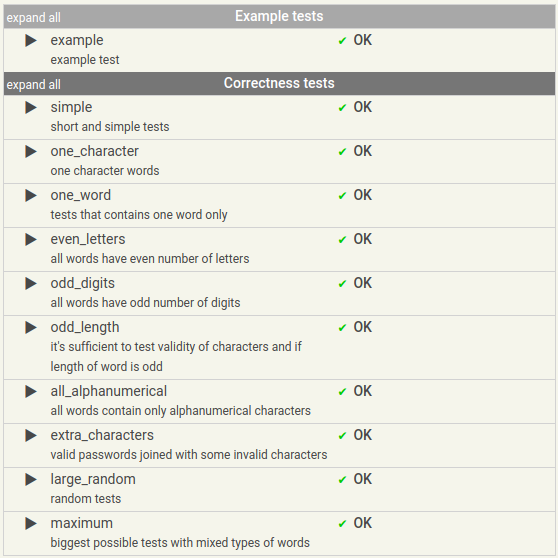
\includegraphics[width=0.8\textwidth]{./test_result.png}
\end{center}

    对不同情况下测试结果均准确,满足设计要求。

    \section{结论}
    从测试结果可以看到,实验程序设计满足要求。程序能够保证输出结果的准确性;程序时间复杂度为线性时间,即使在输入较复杂的情况下仍然能够较快输出结果;程序遍历字符串而非使用切片操作复制为多个字符串,保证了较低的空间复杂度;程序可读性和可维护性均较强。

    设计结果满足设计要求。

    \section{附录}
    \subsection{项目要求原文}
    \input{problem.md}

    \subsection{项目代码}
\begin{lstlisting}
/*************************************************************************
    > File Name: longestpassword.c
    > Author: ShiGuangzhao
    > Mail: Guangzhao_Shi@163.com 
    > Created Time: 2019年12月02日 星期一 21时34分10秒
 ************************************************************************/

#include <stdbool.h>
#include <stdio.h>

int solution(char *S) {
    int MaxLength = 0;
    int CharCount = 0;
    int NumberCount = 0;
    bool PassWord = true;
    for(int i = 0; S[i] != 0; i++) {
        // 0--48, 9--57; A--66, Z--90; a--97, z--122, 空格--32
        // 遇到空格或此字符串不合法
        if(PassWord && S[i] != ' ') {
            if(S[i] <= '9' && S[i] >= '0') {
                NumberCount++;
            }
            else if((S[i] >= 'a' && S[i] <= 'z') \
                    || (S[i] >= 'A' && S[i] <= 'Z')) {
                CharCount++;
            }
            else {
                PassWord = false;
                NumberCount = 0;
                CharCount = 0;
            }
        }
        else {
            // 合法字符串遇到空格
            if(PassWord) {
                if(MaxLength < NumberCount + CharCount \
                        && NumberCount % 2 == 1 \
                        && CharCount % 2 == 0)
                    MaxLength = NumberCount + CharCount;
                NumberCount = 0;
                CharCount = 0;
                PassWord = true;
            }
            // 不合法字符串空格
            else if(S[i] == ' ') {
                PassWord = true;
            }
            // 不合法字符串非空格
        }
    }

    // 最后一个字符串是否合格
    if(PassWord) {
        if(MaxLength < NumberCount + CharCount \
                && NumberCount % 2 == 1 \
                && CharCount % 2 == 0)
            MaxLength = NumberCount + CharCount;
    }
    return MaxLength == 0? -1 : MaxLength;
}

int main(void) {
   char str[] = "test aa1 a0A pass007 ?xy1";
   printf("%s\n", str);
   printf("%d\n", solution(str));
   return 0;
}
\end{lstlisting}

\end{spacing}
\end{document}

